\documentclass[%
 reprint,
%superscriptaddress,
%groupedaddress,
%unsortedaddress,
%runinaddress,
%frontmatterverbose, 
%preprint,
%preprintnumbers,
%nofootinbib,
%nobibnotes,
%bibnotes,
 amsmath,amssymb,
 aps,
%pra,
%prb,
%rmp,
%prstab,
%prstper,
%floatfix,
]{revtex4-2}

\usepackage{graphicx}% Include figure files
\usepackage{dcolumn}% Align table columns on decimal point
\usepackage{bm}% bold math
\usepackage{amsmath}
\usepackage{siunitx}

\preprint{APS/123-QED}
\begin{document}
\title{When ionized oil proved quantization:\\ Data analysis techniques in ionized drops of oil for determining electron charge  }
\author{Braedon Larsen}

\affiliation{Department of Physics and Astronomy \\ Carthage College, Kenosha WI, USA}

\date{January 2026}

\begin{abstract}
The charge on a electron is also refereed to as the elementary charge $e$ and is the quanta for the charge on a particle. Because of the quantization, charge on a particle will be a integer multiple of the elementary charge. By recording the velocities of ionized oil drop when naturally falling, and when under the influence of a known electric field. Normalizing these charges their existence as integer multiples of a single value can be seen. This value is the elementary charge and through the analysis done in this report was found to be $e = (1.569 \pm .0913) \times 10^{-19} \text{C}$
\end{abstract}

\maketitle

\section{Introduction}
Charge is a fundamental property of matter that governs how that matter interacts with electric forces such as electric or magnetic fields. Greater charges lead to increasing effects that EM-fields have on any particular particle. In 1897, physicist J.J Thomson had discovered the existence of a charged particle that is known as the electron\cite{thomson}. Thomson had also quantified the ratio of the charge of this electron to its mass, but no measurement of its charge or its mass existed yet. However, about a decade after Thomson's initial measurement, there were many scientists taking different approaches in attempting to quantify either the mass or the charge of the electron. The first to succeed was Robert Millikan who quantified the charge of electron, and since the ratio of the electrons charge to mass was known, he also quantified the mass of a electron. His experiment, now known as the "Millikan Oil Drop Experiment" took a different approach to many others, relying on fluid mechanics and the net forces exerted on a particle. Millikan used small drops of oil, so small that the viscosity of air made them fall at a constant observable rate. Using a source of ionizing radiation, a random net charge is applied to the oil drop. If these charges can be determined for a statistically sufficient number of oil drops. The differences between the charges could be taken, from these differences, a pattern emerged where the differences were all a integer multiple of a minimum charge difference. This result verified the theory that charge was a quantized value and that quanta was the charge of a electron. In one experiment Millikan verified the charge of a electron which is now called $e$ or the elementary charge, and that the elementary charge is the smallest unit of charge that is possible. 
\\
For this report, the experiment Millikan preformed will be replicated and analyzed using modern data analysis techniques for both verifying the value of the elementary charge and the nature of charge as a quantized quantity. 



\section{Methodology and Results}
For experimentation, a AP-8210 \cite{pascoap8210}, was used with Squibb\#5597 as the mineral oil \cite{squibb}, and Thorium-232 \cite{pascoap8210} as the source of ionizing radiation. After calibration of the apparatus, multiple attempts for data collection were preformed. 
\\
The AP-8210 consisted of a small chamber enclosed on all sides but for a small hole in the cap, the upper and lower walls of the chamber were the plates of a capacitor, and the sides a plastic spacer. The hole was used in combination with a atomizer to spray small drops of oil into the chamber that could then be briefly exposed to the ionizing radiation before testing. The bubbles were viewed through a 30x magnification scope with a reticle marking every $.5$mm and $.1$mm.
\\
For each of these attempts, oil drops were introduced to the viewing chamber and ionized, the drops were then evaluated to select a drop that both: reacted to the polarities of the capacitor, and naturally fall at a appreciable rate. After a proper drop was selected, the bubble was timed for its time to travel $.5$ mm in 3 configurations: falling naturally, rising with positive top plate polarity, and falling with negative top plate polarity. 
\\
Between all runs 3 drops were found to meet these criteria, and for these 3 drops, 6 ionization states were achieved. The additional states were achieved by re-ionizing the same drop after the first runs of data were collected. For these re-ionizations, the natural falling velocity was unchanged as the drop had nearly the same mass (any mass loss or gain due to gaining or losing charged particles is negligible).

To find the charge in a oil drop, we begin with free body diagrams for the potential states that the drop can be in. The drop has a net charge $q$, which will be affected by an electrostatic force when there is polarity on the plates. 
As can be seen in \ref{fig:FBDs}, the two cases are with field polarity or no field polarity. The two cases are considered to enter equilibrium instantaneously on the timescales used, the forces will balance and create the following equations
\begin{figure}[h!]
    \centering
    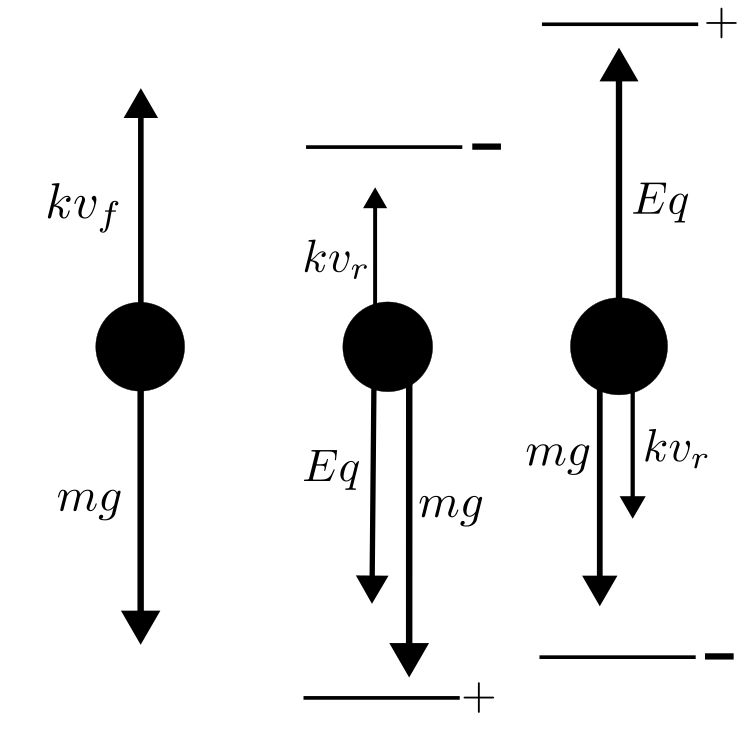
\includegraphics[width=1\linewidth]{polarityFBD_V1.png}
    \caption{Free body diagrams of the 3 potential states for the oil drop. Leftmost is the neutral state with the only forces being gravity and drag, the middle is the top plate negative state where the electric field causes a downwards force on the bubble, and the right is the top plate positive state causing the bubble to move upwards against gravity}
    \label{fig:FBDs}
\end{figure}

\begin{align}
    \text{For no field polarity: } mg &= k v_f \label{noPolEq} \\
    \text{For top plate + charged field: } Eq &= mg+kv_r \label{polEq} \\
    \text{For top plate - charged field: } Eq + mg &= kv_r
\end{align}
Where $m$ is the mass of the droplet, $g$ is acceleration due to gravity, $v_f$ is the terminal velocity when the drop naturally falls, $v_r$ is the terminal velocity when the drop is under the influence of the electric field, $k$ is the coefficient of drag, and $E$ is the electric field strength. 
Solving \eqref{noPolEq} and \eqref{polEq} for $q$ yields the following:
\begin{align}
    q = \frac{mg(v_f+v_r)}{Ev_f} \label{mq}
\end{align}
The mass of the drop can be expanded using the density $\rho$ of the oil 
\begin{align}
    m = \frac{4}{3}\pi a^3\rho
\end{align}
Where $\rho$ is the density of the oil, and $a$ is the radius of the drop. 
The radius of the drop $a$ can be further expanded using Stoke's Law relating the radius of a sphere and its velocity when falling in a viscous medium. 
\begin{align}
    a = \sqrt{\frac{b}{2{P}}^2+\frac{9\eta v_f}{2g\rho}-\frac{b}{2P}}
\end{align}
Where $b$ is a constant equal to $b = 8.2 \times 10^{-3} \text{Pa} \cdot \text{m}$, $P$ is the pressure of the environment, and $\eta$ is the viscosity of air.
\\
This term for $a$ can be substituted into \eqref{mq} and simplified to the final form of:
\begin{align}
    q = \frac{4}{3}\pi \rho g \Bigg[\sqrt{\frac{b}{2P}^2+\frac{9\eta v_f}{2g\rho}}-\frac{b}{2P}\Bigg]^3\frac{v_f+v_r}{Ev_f}
    \label{bigQ}
\end{align}


After collecting the data, several processes were in the data analysis. This process will be covered briefly here but is explained in greater detail in the supplemental information \cite{supp}. For each of the charge states, an averaged falling velocity $\bar{v_f}$, an averaged positive rising velocity $\bar{v_{+}}$, and an averaged negative rising (falling) velocity $\bar{v_-}$. With these velocities for each of the 6 charge states, they were then used with \eqref{bigQ} to calculate a net charge for each charge state for the position and negative cases. 
\\
These positive and negative charges were averaged to get a single charge value for each charge state $q_i$. These charge states were then normalized by the smallest charge state, then the normalized charges were multiplied by the integer that yielded a minimum total distance of each normalized charge from its nearest integer neighbor. This is because as charge is quantized, the values for charge on a particle should follow a integer multiple of the fundamental charge, this methods working to find what the integer multiples are in the data. To verify the distance to the nearest integer, a trial and error method was used since there was so few integers to check (1-11). The "ideal integer", was selected by which integer brought the dataset closest to a least squares fit line. The results of this fitting can be seen in \ref{fig:qvsNPLot} and the final linear equation found whose slope is equivalent to the fundamental charge.
\begin{figure}[h]
    \centering
    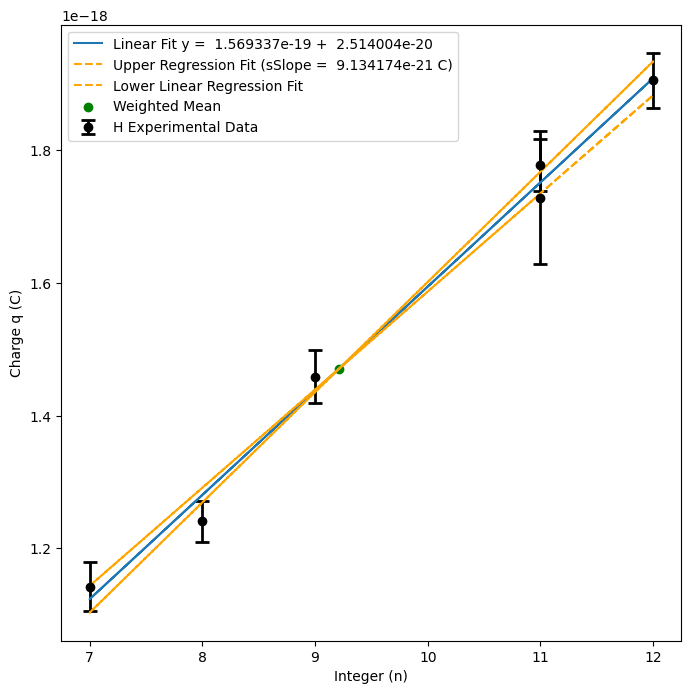
\includegraphics[width=1\linewidth]{qVsNPlot_V1.png}
    \caption{Charge vs n-integer plot, used to find the best estimate for the charge of a electron $e$. The linear best fit line's slope is equivalent to $e$, with the linear best fit following the linear equation $y = (1.881 \pm .205) \times 10^{-19} + 1.149 \times 10^{-20}$. In addition the plot shows the points of experimental data, the weighted mean, and a visualization of the error to the slope.}
    \label{fig:qvsNPLot}
\end{figure}
\newpage
From \ref{fig:qvsNPLot}, a refined estimate for the value of $e$ is obtained as the slope of the linear least squares fit on that plot. This value was found to be $e = (1.569 \pm .0913) \times 10^{-19} \text{C}$. Compared to the accepted value from NIST ($e = 1.602e-19$C) \cite{NIST_CODATA}, there is a z-score of .357 and the best value itself is within 1.9\% of the accepted value. The z-score value implies that the range calculated is within .357 standard deviations of the dataset to the "mean" or in this case accepted value being a underestimate by the positive sign for the z-score. It is clear in this case that the methodology of the experiment preform properly. With the observed values 
 




\section{Conclusions}
In summary, the use of droplets small enough that air behaves viscous to them. Allows measuring their velocity to be used for calculated charge on the particles when ionized to react to an electric field, and by consequence of charge quantization, calculate the fundamental charge $e$. After collecting a data set of velocities, a several step data analysis process was preformed to go from the collected drop velocities to the charge on each drop. Once the charge for each drop was obtained, the data was fitted using the theory that charge was quantized and the charge values would be integer multiples of the fundamental charge. This analysis lead to a final value for the fundamental charge of  $e = (1.569 \pm .0913) \times 10^{-19} \text{C}$. This value, is consistent with the accepted value .
For a greater certainty to the value, more data points per charged state could be used. Using a larger dataset with provide more evidence for the quantization of charge by showing the smallest difference that charged particles could have between their charges. 


\section*{Acknowledgments}
The author would like to acknowledge Sema'je Farmer for his assistance with the data collection involved for this experiment. 

\section*{Data Availability Statement}
A Jupyter notebook containing all the experimental data, data analysis, figure generation, and additional information on uncertainty analysis can be found in the supplemental materials. \cite{supp}
\bibliography{biblo}

\end{document}
